\documentclass[11pt,]{article}
\usepackage[left=1in,top=1in,right=1in,bottom=1in]{geometry}
\newcommand*{\authorfont}{\fontfamily{phv}\selectfont}
\usepackage[sc, osf]{mathpazo}


  \usepackage[T1]{fontenc}
  \usepackage[utf8]{inputenc}



\usepackage{abstract}
\renewcommand{\abstractname}{}    % clear the title
\renewcommand{\absnamepos}{empty} % originally center

\renewenvironment{abstract}
 {{%
    \setlength{\leftmargin}{0mm}
    \setlength{\rightmargin}{\leftmargin}%
  }%
  \relax}
 {\endlist}

\makeatletter
\def\@maketitle{%
  \newpage
%  \null
%  \vskip 2em%
%  \begin{center}%
  \let \footnote \thanks
    {\fontsize{18}{20}\selectfont\raggedright  \setlength{\parindent}{0pt} \@title \par}%
}
%\fi
\makeatother




\setcounter{secnumdepth}{0}


\usepackage{graphicx}
% We will generate all images so they have a width \maxwidth. This means
% that they will get their normal width if they fit onto the page, but
% are scaled down if they would overflow the margins.
\makeatletter
\def\maxwidth{\ifdim\Gin@nat@width>\linewidth\linewidth
\else\Gin@nat@width\fi}
\makeatother
\let\Oldincludegraphics\includegraphics
\renewcommand{\includegraphics}[1]{\Oldincludegraphics[width=\maxwidth]{#1}}

\title{What Americans Really Think About Gun Control: Evidence from the General
Social Survey, 1972-2016 \thanks{Replication files are available on the author's Github account
(\href{https://github.com/svmiller}{github.com/svmiller}).
\textbf{Corresponding author}:
\href{mailto:svmille@clemson.edu}{\nolinkurl{svmille@clemson.edu}}.}  }



\author{\Large Steven V. Miller\vspace{0.05in} \newline\normalsize\emph{Clemson University}  }


\date{}

\usepackage{titlesec}

\titleformat*{\section}{\normalsize\bfseries}
\titleformat*{\subsection}{\normalsize\itshape}
\titleformat*{\subsubsection}{\normalsize\itshape}
\titleformat*{\paragraph}{\normalsize\itshape}
\titleformat*{\subparagraph}{\normalsize\itshape}


\usepackage{natbib}
\bibliographystyle{apsr}
\usepackage[strings]{underscore} % protect underscores in most circumstances



\newtheorem{hypothesis}{Hypothesis}
\usepackage{setspace}

\makeatletter
\@ifpackageloaded{hyperref}{}{%
\ifxetex
  \PassOptionsToPackage{hyphens}{url}\usepackage[setpagesize=false, % page size defined by xetex
              unicode=false, % unicode breaks when used with xetex
              xetex]{hyperref}
\else
  \PassOptionsToPackage{hyphens}{url}\usepackage[unicode=true]{hyperref}
\fi
}

\@ifpackageloaded{color}{
    \PassOptionsToPackage{usenames,dvipsnames}{color}
}{%
    \usepackage[usenames,dvipsnames]{color}
}
\makeatother
\hypersetup{breaklinks=true,
            bookmarks=true,
            pdfauthor={Steven V. Miller (Clemson University)},
             pdfkeywords = {gun control, political attitudes, public opinion, polarization, elite
cues},  
            pdftitle={What Americans Really Think About Gun Control: Evidence from the General
Social Survey, 1972-2016},
            colorlinks=true,
            citecolor=blue,
            urlcolor=blue,
            linkcolor=magenta,
            pdfborder={0 0 0}}
\urlstyle{same}  % don't use monospace font for urls

\linespread{1.05}


% add tightlist ----------
\providecommand{\tightlist}{%
\setlength{\itemsep}{0pt}\setlength{\parskip}{0pt}}

\begin{document}
	
% \pagenumbering{arabic}% resets `page` counter to 1 
%
% \maketitle

{% \usefont{T1}{pnc}{m}{n}
\setlength{\parindent}{0pt}
\thispagestyle{plain}
{\fontsize{18}{20}\selectfont\raggedright 
\maketitle  % title \par  

}

{
   \vskip 13.5pt\relax \normalsize\fontsize{11}{12} 
\textbf{\authorfont Steven V. Miller} \hskip 15pt \emph{\small Clemson University}   

}

}








\begin{abstract}

    \hbox{\vrule height .2pt width 39.14pc}

    \vskip 8.5pt % \small 

\noindent Gun control is one of the most controversial public opinion debates in
the United States with each new mass shooting raises the stakes involved
in the debate. It is easy to assume gridlock that has blocked
legislation on gun control follows because of the mass-level
polarization on the topic of gun control. My analysis of 28 waves of
General Social Survey data from 1972 to 2016 shows this is wrong. My
analysis of the data generates four key findings: 1) GOP partisanship
does not robustly reduce support for gun control; 2) most `strong'
Republicans actually support gun control; 3) polarization of attitudes
about gun control is only partial and recent; and 4) our casual
assumptions about regional variation in attitudes toward gun control
need re-evaluation. I conclude with a discussion of the differences we
observe between elite polarization and mass polarization and with
implications for the future of gun control advocacy.


\vskip 8.5pt \noindent \emph{Keywords}: gun control, political attitudes, public opinion, polarization, elite
cues \par

    \hbox{\vrule height .2pt width 39.14pc}



\end{abstract}


\vskip 6.5pt


\noindent  \section{Introduction}\label{introduction}

Gun control is one of the most controversial public policy issues in the
United States. Its salience has only increased after recent domestic
terror incidents in places like the Pulse night club and the Inland
Regional Center in San Bernardino. The San Bernadino incident in
particular led to a strong reaction from some leading newspapers trying
to push this debate into legislative action. The \emph{New York Daily
News} ran a front-page cover that engaged in deliberate issue linkage of
the San Bernardino incident with other semi-automatic rampages in
Aurora, Colorado Springs, and Newtown, labeling all as ``terrorists''
\citep{nydn2015ht}. The \emph{New York Times} even dusted off a device
it had not used in 95 years---the front-page editorial---to argue that
legislative unwillingness to push sensible gun control legislation into
law is a ``moral outrage and national disgrace'' \citep{nyt2015egea}.
Successive incidents since, prominently the October 2017 mass shooting
in Las Vegas that now ranks as the deadliest individual act of mass
murder in U.S. history, only raise more questions about our gun laws and
the salience of this controversial public policy debate. The
demonstrations by the \emph{New York Daily News} and \emph{New York
Times} still resonate among gun control advocates in light of more
current events.

The \emph{New York Daily News} and \emph{New York Times} made these
demonstrations because gun control legislation is a non-starter in
Congress. The day after the San Bernardino incident, Senate Republicans
voted down legislation that would have closed background check loopholes
and banned subjects on the terror watch list from purchasing firearms
\citep{joseph2015srvd}. Republican opposition was almost unanimous,
which conforms to the preferences of the National Rifle Association
(NRA) on this issue. The implication here is Republican opposition to
any gun control legislation follows the direct preferences of its core
interest groups and its constituents. In a heavily polarized political
climate, gun control legislation is a non-starter as long as Republicans
control Congress or are in a position to filibuster gun control
legislation. This speaks well to political science scholarship that says
public opinion \citep[e.g.][]{pageshapiro1983epop}, especially on
salient issues \citep{burstein2003ipo}, drives public policy in the
United States.

My analysis of a 44-year span of General Social Survey data tells a
mixed story of the conventional wisdom that Republican leaders block gun
control legislation because Republican voters are against it. I find
that Republican partisanship does not robustly reduce support for gun
control and that most Republicans actually support gun control. Gun
control is not necessarily a partisan issue over time even if it has
quickly become one. I also find that the American West, not the South,
is where support for gun control is the lowest. I conclude that there is
still substantial support for even meaningful gun control legislation
and that a lot of conventional wisdom about gun control merits
re-evaluation.

\section{Methods}\label{methods}

I use General Social Survey (GSS) data for all available years from 1972
to 2016. The primary question of interest---whether the respondent
favors or opposes a law that would require a person to obtain a police
permit before he or she could buy a gun---is the most ubiquitous gun
control item in the GSS. Its utility for the sake of this analysis is
multiple. One, it appears in 28 of the 31 available GSS waves from 1972
to 2016.\footnote{The question was not asked in 1978, 1983, or 1986.}
Other gun control items that appear in GSS are one-time questions. Two,
the substance of the gun control question that GSS asks is subtly
aggressive. It prompts the respondent to ask whether state approval for
a gun of any kind is necessary when gun control opponents tend to cite
precisely this kind of state overreach as justification for a maximalist
interpretation of the Second Amendment to the U.S. Constitution. Thus,
gun control advocates and interested lawmakers in Washington almost
never express a gun control proposal like this, instead preferring to
massage objections from gun control opponents with policies that target
gun show loopholes, terror watch lists, or military-style rifles like
the AR-15. GSS respondents that favor this form of gun control are
signaling their willingness to accept other aggressive gun control
measures. I keep the binary nature of this variable where a 1 indicates
support of this form of gun control.

I also select data from the 2006 wave that features more granular
questions about gun control policies. These include background checks
for private sales, tougher penalties for illegal gun sales than drug
sales, limiting semi-automatic weapons the police and military, making
it illegal to carry a gun while drunk, and support for tougher gun
control legislation as a function of the 9/11 terrorist attacks. These
are binary variables that assume a value of 1 for respondents that favor
a more aggressive gun control proposal.

The primary independent variable of interest is partisanship. This is
the familiar seven-point partisanship question that ranges from ``strong
Democrat'' to ``strong Republican.'' I also include variables for age,
sex (female), whether the respondent has a college education, fixed
effects for race (leaving whites as the baseline), and whether the
respondent has a gun in the household.

All dependent variables are binary, making the use of a logistic
regression appropriate. However, there is important spatial and temporal
heterogeneity across the 28 waves of GSS data that I use in my analysis.
I account for this with mixed effects models with random effects for the
condensed Census region in which the respondent resides and, for the
primary dependent variable, the year of the survey. I allow the effect
of partisanship to vary by region and condensed Census region. I also
scale all non-binary independent variables by two standard deviations to
ensure rough comparability of coefficients \citep{gelman2008sri}.

\section{Results}\label{results}

My analyses of 28 waves of GSS data over 44 years suggest four
interesting findings about public opinion and the gun control debate.
First, partisanship with the Republican party does not robustly reduce
support for gun control. Second, most Republicans actually support gun
control, even in the current polarized political climate. Third, gun
control is not necessarily a partisan issue but it is quickly becoming
one. Finally, simple assumptions about regional variation mask important
and more intriguing variation on attitudes toward gun control in the
data.

\subsection{Partisanship Does Not Robustly Reduce Support for Gun
Control}\label{partisanship-does-not-robustly-reduce-support-for-gun-control}

Partisanship might be our go-to explanation for individual-level support
for gun control. The implication is increasing identification with the
Republican Party decreases support for gun control given the many cues
Republican elites send to their voters about gun control
\citep[c.f.][]{zaller1992nomo}. However, the partisanship-gun control
relationship is not nearly as robust at the individual-level as we infer
it to be at the elite-level.

\begin{table}[!htbp] \centering 
  \caption{Mixed Effects Models of Attitudes toward Gun Control} 
  \label{} 
\small 
\begin{tabular}{@{\extracolsep{5pt}}lcccccc} 
\\[-1.8ex]\hline \\[-1.8ex] 
\\[-1.8ex] & \emph{} & \emph{Background} & \emph{Tougher} &
                \emph{} & \emph{ } & \emph{Tougher} \\
\\[-1.8ex] & \emph{Require} & \emph{Check for} & \emph{ Penalties} &
                \emph{Limit} & \emph{Illegal to} & \emph{Gun} \\
\\[-1.8ex] & \emph{Police} & \emph{Private} & \emph{than} &
                \emph{Semi-} & \emph{Carry Gun} & \emph{Control} \\
\\[-1.8ex] & \emph{Permit} & \emph{Sales} & \emph{Drugs} &
                \emph{Automatics} & \emph{While Drunk} & \emph{After 9/11} \\
\\[-1.8ex] & \textbf{Model 1} & \textbf{Model 2} & \textbf{Model 3} & \textbf{Model 4} & \textbf{Model 5} & \textbf{Model 6}\\ 
\hline \\[-1.8ex] 
 Age & 0.101$^{*}$ & $-$0.051 & 0.356$^{*}$ & 1.278$^{*}$ & 0.170 & 0.073 \\ 
  & (0.027) & (0.188) & (0.152) & (0.260) & (0.267) & (0.223) \\ 
  College Educated & 0.345$^{*}$ & 0.598$^{*}$ & $-$0.162 & 0.457 & 0.349 & 0.113 \\ 
  & (0.035) & (0.231) & (0.168) & (0.283) & (0.317) & (0.252) \\ 
  Female & 0.644$^{*}$ & 0.955$^{*}$ & 0.109 & 2.041$^{*}$ & 0.628$^{*}$ & 1.219$^{*}$ \\ 
  & (0.027) & (0.186) & (0.150) & (0.264) & (0.256) & (0.217) \\ 
  Black & 0.118$^{*}$ & $-$0.253 & 0.884$^{*}$ & 0.547 & $-$0.515 & $-$0.191 \\ 
  & (0.044) & (0.291) & (0.242) & (0.438) & (0.389) & (0.378) \\ 
  Other Race (Not White) & 0.342$^{*}$ & $-$0.202 & 0.873$^{*}$ & 1.045$^{*}$ & $-$0.396 & 0.342 \\ 
  & (0.071) & (0.332) & (0.279) & (0.472) & (0.417) & (0.425) \\ 
  Party ID (D to R) & $-$0.407$^{*}$ & $-$0.288 & 0.083 & $-$0.366 & $-$0.292 & $-$0.567$^{*}$ \\ 
  & (0.066) & (0.209) & (0.173) & (0.250) & (0.347) & (0.280) \\ 
  Gun in the Household & $-$0.963$^{*}$ & $-$0.529$^{*}$ & $-$0.603$^{*}$ & $-$1.288$^{*}$ & $-$0.063 & $-$1.198$^{*}$ \\ 
  & (0.028) & (0.191) & (0.160) & (0.245) & (0.277) & (0.221) \\ 
\hline 
 N & 35,972 & 838 & 835 & 832 & 842 & 790 \\ 
\hline \\[-1.8ex] 
\multicolumn{7}{l}{\scriptsize $^{*}$p $<$ .05} \\ 
\multicolumn{7}{l}{\scriptsize \emph{Random effect parameters (i.e. slope and intercept standard deviations) omitted for presentation.}} \\ 
\end{tabular} 
\end{table}

Table 1 summarizes the results from six mixed effects regression models
on the dependent variables I coded from the GSS data. Increasing
partisanship with the Republican Party does not have robust effects
across all six models. Increasing GOP partisanship reduces support for a
law that would require a police permit to own a gun and reduces support
for tougher gun control laws when gun control is deliberately linked to
terror threats after 9/11. However, increasing Republican partisanship
does not have a discernible effect on attitudes toward background checks
for private sales, tougher penalties for illegal gun purchases than
illegal drug sales, limiting semi-automatics to the police and military,
and for making it illegal to carry a gun while drunk.

Republican partisanship might be the easiest way of thinking about
opposition to gun control legislation in the United States but GSS data
suggest the effect of Republican partisanship on attitudes toward gun
control measures is not robust across multiple forms of gun control
policies.

\subsection{Most Republicans Actually Support Gun
Control}\label{most-republicans-actually-support-gun-control}

Perhaps the most counterintuitive finding from survey data on attitudes
toward gun control is that Republicans generally favor gun control
legislation. This is not an anomaly unique to a specific year, nor
necessarily a recent trend. There is not a year in the 28 waves of GSS
data in which support among \emph{strong} Republicans for a law that
would require a police permit for a gun purchase is below 50\%.

\begin{figure}[htbp]
\centering
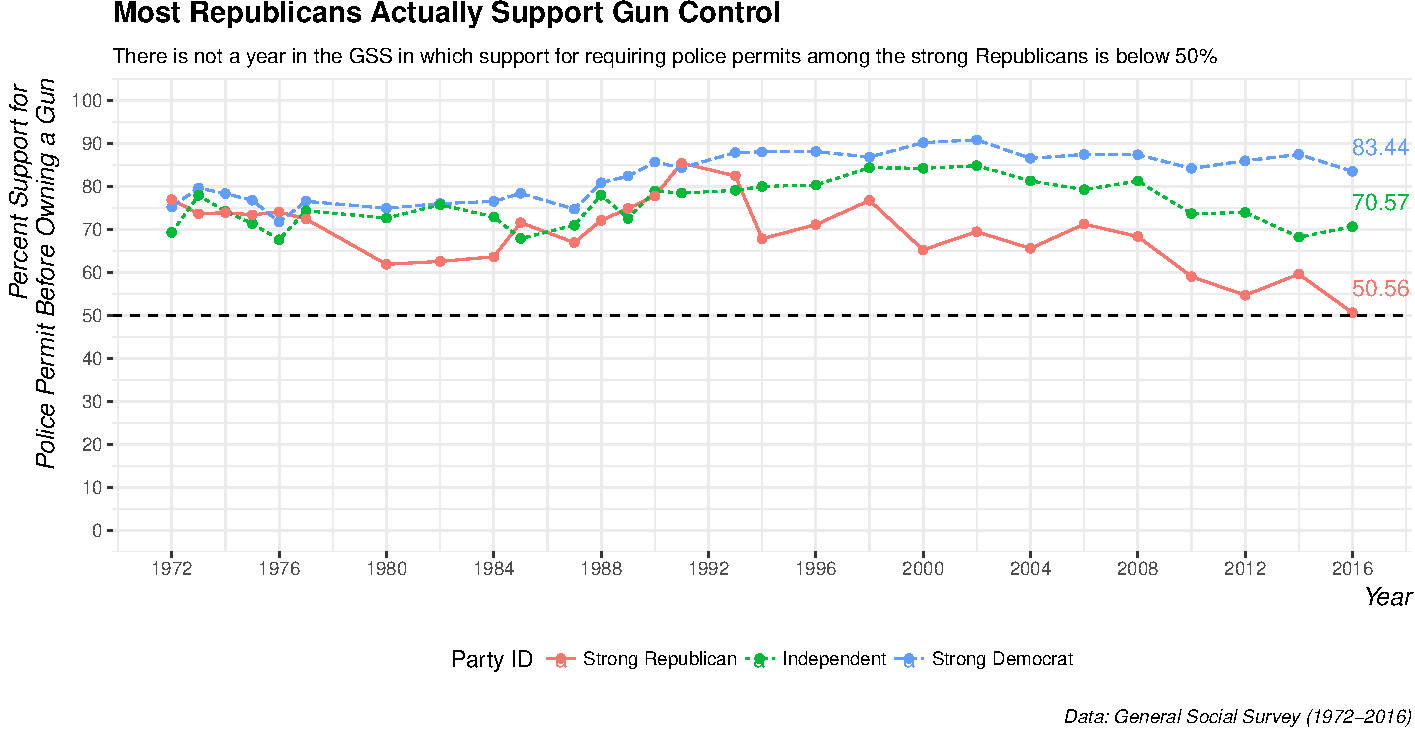
\includegraphics{gss-guns_files/figure-latex/ts1-1.pdf}
\caption{Support for Gun Control among Partisans Over Time}
\end{figure}

Figure 1 is a time-series line chart of the percentage of responses that
favor a law requiring a police permit before a person could buy a gun by
partisan identification over the 27 waves from 1972 to 2016 in which
that item appears. For clarity, I subset the line chart to just the
strong Democrats, the independents who do not lean toward either party,
and the strong Republicans. The line chart shows that the lowest support
for this form of gun control came in 2012, in which 54.62\% of strong
Republicans favored this form of gun control. Support among the strong
Republicans actually increased almost five percentage points to 59.54\%
in the two years after the 2012 survey, though fell again to 50.5\% in
2016.

Figure 1 does show some other interesting trends over the years. Strong
Democrats have become only a little more supportive of gun control over
time. 75.16\% of strong Democrats favored this gun control measure in
1972, which increased to 83.44\% in 2016. Independents who do not lean
toward one party have not changed over time. In 1972, support for this
form of gun control was 69.23\% among those independents, relative to
70.57\% in 2016. Interestingly, strong Republicans tracked quite closely
with strong Democrats before 1994. The year of the ``Republican
Revolution'', in which the GOP took both chambers of Congress for the
first time since 1953, saw support for this form of gun control fall
from 82.4\% in 1993 to 67.77\% in 1994.

\begin{table}[!htbp] \centering 
  \caption{Expected Values of Support for Police Permits for Gun Purchases Among Strong Republicans} 
  \label{} 
\begin{tabular}{@{\extracolsep{5pt}} ccc} 
\\[-1.8ex]\hline 
\hline \\[-1.8ex] 
Category & Expected Value & 95\% Interval \\ 
\hline \\[-1.8ex] 
Female, Doesn't Own Gun & .836 & (.789, .874) \\ 
Male, Doesn't Own Gun & .728 & (.662, .786) \\ 
Female, Gun Owner & .661 & (.591, .729) \\ 
Male, Gun Owner & .507 & (.430, .585) \\ 
Male, Gun Owner, College Educated & .592 & (.512, .665) \\ 
\hline \\[-1.8ex] 
\end{tabular} 
\end{table}

Figure 1 clarifies the results from Model 1, telling us that strong
Republicans are less likely to support gun control but this should not
be confused as equivalent to a statement that strong Republicans are
likely to ``oppose'' gun control. Table 2 tells a similar story with
simulations of the regression from a multivariate normal distribution to
generate quantities of interest. I set the explanatory variables at
their typical values (i.e.~white respondents around age 51 without a
college education), set the party ID variable at its maximum
(i.e.~strong Republicans) and allow the gun ownership and gender
variable to vary. The simulations show the point estimates for expected
value of support for police permits for gun purchases, given the
explanatory variables (e.g.~women/men, strong GOP, owns gun/does not own
a gun) are above .500 in every application. Further, the 95\% interval
for all expected values from the simulations are above .500 in all but
one category: men with strong GOP affiliation, no college education, and
with a gun in the home. However, one adjustment to that class of
respondent---the presence of a college diploma---increases support for
police permits before purchasing a gun to .592 with a 95\% distribution
of expected values that are above .500.

This is an important pedagogical lesson for pundits, scholars, and
interested citizens who want to understand variation in public opinion
about the gun control debate. Model 1 in Table 1 shows a negative
relationship between increasing GOP partisanship and support for a
police permit prior to owning a gun that is discernible from a zero
relationship. In other words, increasing partisanship with the
Republican party decreases support for this form of gun control relative
to those with lesser affinity for the GOP (including strong Democrats).
The reader can mostly see this story in Figure 1. However, it would be a
mistake, both statistical and substantive, to assume that statement is
equivalent to ``increasing GOP partisanship makes a respondent oppose
this form of gun control.'' This would not be true in this case. Strong
Republicans still support this form of gun control, though strong
Democrats support it more.

\subsection{Gun Control Is Not Necessarily a Partisan Issue, but It Is
Becoming
One}\label{gun-control-is-not-necessarily-a-partisan-issue-but-it-is-becoming-one}

Most Republicans are on board with gun control measures. However, we are
observing a growing rift between Democrats and Republicans on this issue
that seems to have increased during the Obama Administration.

Figure \ref{fig:simyear} shows more simulations of the dependent
variable from a draw of a multivariate normal distribution for three
different values of partisanship---strong Republicans, strong Democrats,
and pure independents---across all survey waves with all other
explanatory variables held at their typical value. The results show
partisan differences first emerging as a result of the Republican
Revolution of 1994 but show increasing polarization on this issue that
seems to occur almost entirely during the Obama Administration. This
coincides with prominent events like the spike in gun sales after
Obama's 2008 election \citep{bohn2008gss} and cues from the NRA that
Obama was the most ``anti-gun candidate ever'' who will ``take your guns
away'' \citep{smith2008nra}. On average, Republicans are less likely to
support this gun control measure than those whose political affinities
gravitate more to the Democratic Party. However, Figure
\ref{fig:simyear} shows that the effect of GOP partisanship is more
pronounced in recent years than it is overall.

\begin{figure}[htbp]
\centering
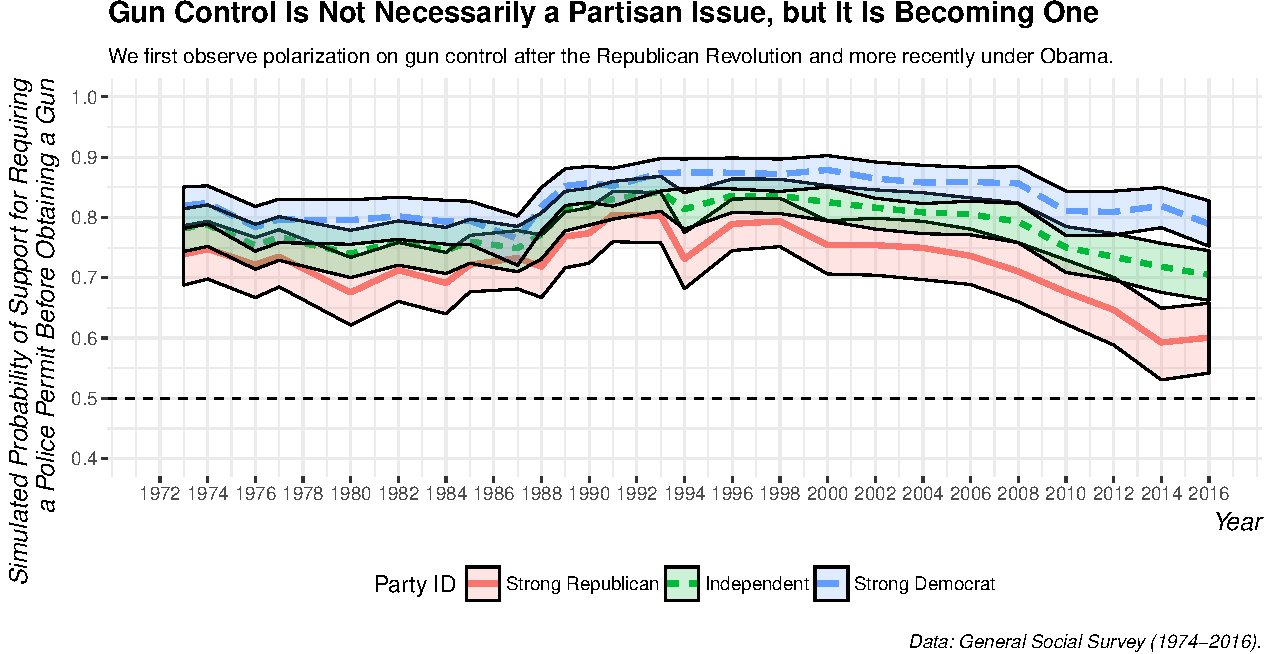
\includegraphics{gss-guns_files/figure-latex/simyear-1.pdf}
\caption{\label{fig:simyear} Support for Gun Control by Year and
Partisanship}
\end{figure}

Most Republicans actually support gun control measures and the issue at
stake is not necessarily as polarizing at the individual-level as it is
at the elite-level. However, it is quickly becoming a partisan issue
among the electorate.

\subsection{Unintuitive Regional and Temporal Variation in Support for
Gun
Control}\label{unintuitive-regional-and-temporal-variation-in-support-for-gun-control}

Explanations for attitudes about gun control across regions in the
United States tend to make rather broad and simple statements.
Southerners love guns, for whatever purpose
\citep[e.g][]{brennanetal1993gsgc}, which we think makes Southerners
more likely to elect politicians who will fight hard for their
interpretation of the Second Amendment to the U.S. Constitution.
Likewise, guns are prominent in the the West as well, which might make
the region also more opposed to gun control in general
\citep{wolpertgimpel1998sisp}.

These statements belie interesting variation in attitudes toward gun
control across regions and by partisanship. Figure \ref{fig:simgoprevol}
summarizes simulations from a split of Model 1 in Table 1, subsetting
the analyses of Model 1 in Table 1 to the survey waves before the
``Republican Revolution'' (1972-1993) and after it (1994-2016).
Thereafter, I generate simulations with confidence intervals for varying
levels of partisanship across the four Census regions in the model with
all other explanatory variables held at their typical value. Figure
\ref{fig:simgoprevol} does not suggest any meaningful variation in
attitudes toward gun control as a result of the sorting of the
electorate in 1994 in the Midwest or the West. Instead, we see two
interesting and discrernible differences in the Northeast and the South.
Republicans in the Northeast are less likely to support gun control
after the Republican Revolution than Republicans in the Northeast before
it. Further, we see a small but discernible difference in the South,
though it involves the strong Democrats and not the strong Republicans.
Strong Democrats in the South became more likely to support gun control
after the Republican Revolution than strong Democrats before it.

\begin{figure}[htbp]
\centering
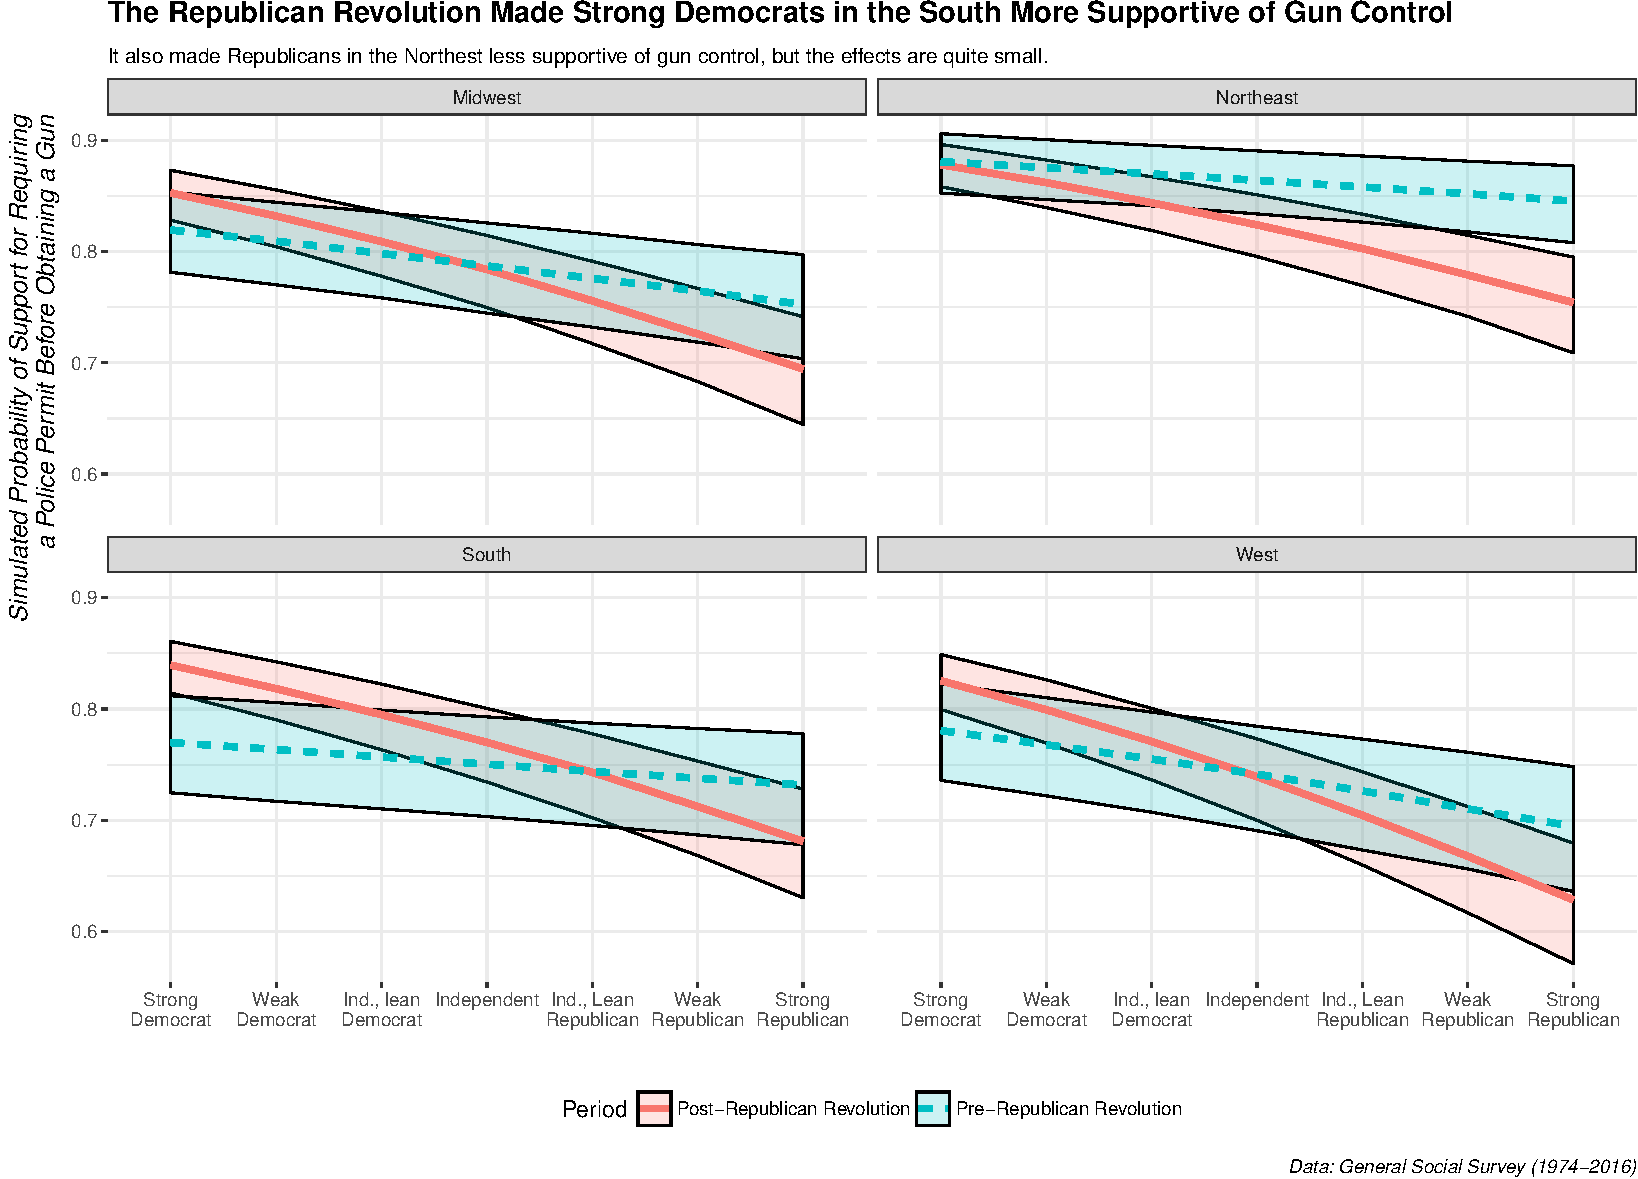
\includegraphics{gss-guns_files/figure-latex/simgoprevol-1.pdf}
\caption{\label{fig:simgoprevol} Support for Gun Control by
Partisanship, Before and After the Republican Revolution}
\end{figure}

Figure \ref{fig:simyearregion} generates simulations of the likelihood
of supporting mandatory police permits before obtaining a gun by
condensed Census region and three values of partisanship: strong
Democrats, strong Republicans, and pure independents who say they do not
lean either way. The results are consistent with the previous discussion
that suggests even strong Republicans support gun control and that gun
control's polarization on partisan lines is only recent. The South is
unique among the four regions here because we cannot discern a
difference between independents and the strong Republicans and strong
Democrats in the more recent survey waves when we factor in the
uncertainty around the simulation's estimates. The simulations for the
three other regions in the most recent survey waves suggest differences
among all three partisan groups with the widest differences among groups
appearing in the West.

\begin{figure}[htbp]
\centering
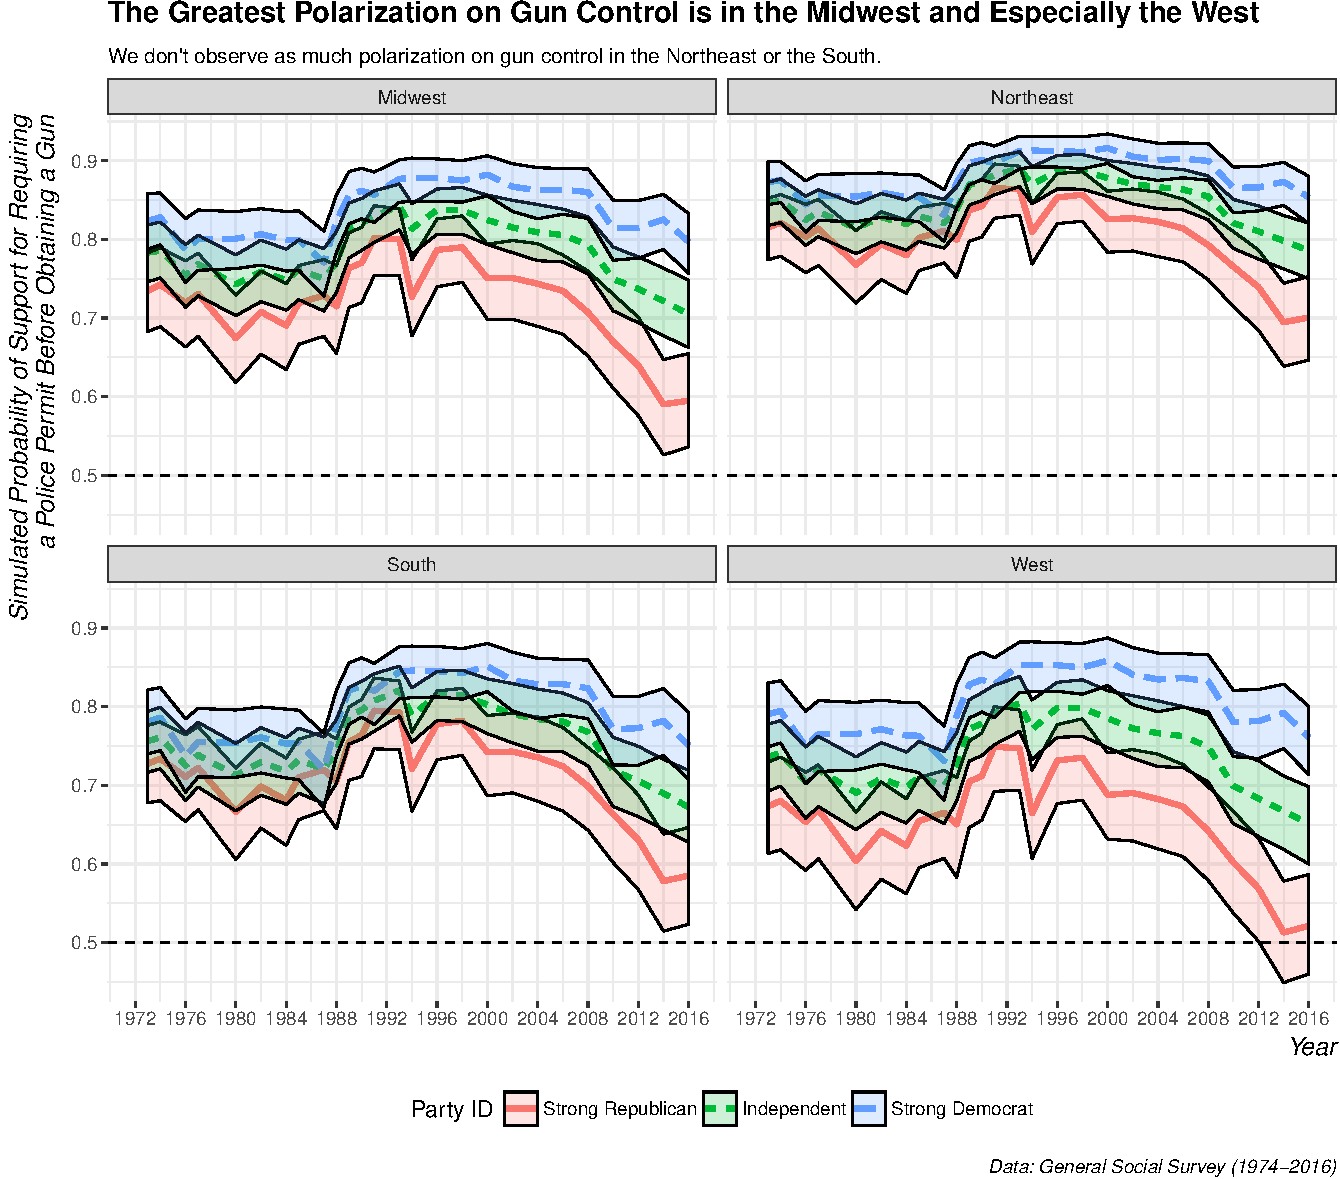
\includegraphics{gss-guns_files/figure-latex/simyearregion-1.pdf}
\caption{\label{fig:simyearregion} Support for Gun Control by
Partisanship and Region}
\end{figure}

All told, there is clear regional variation in attitudes toward gun
control by different values of partisanship and over time. However, the
variation does not fit a simple pattern we otherwise casually assume.
Strong Democrats in the South---and not the region's strong Republicans,
per se---observe a change in attitudes toward gun control after the
Republican Revolution. Changes in attitudes toward gun control in the
Northeast after that sorting of the electorate was more about changes
among Republicans than Democrats. More recent waves have seen
significant partisan sorting on attitudes toward gun control in every
region, though less so in the South.

\section{Conclusion}\label{conclusion}

This study examined Americans' attitudes toward gun control over 28
waves of the GSS data, resulting in four findings that question
conventional wisdom about public opinion in the gun control debate.
First, GOP partisanship does not robustly reduce support for gun
control. Second, most ``strong Republicans'' actually support a subtly
aggressive form of gun control. Third, polarization in the gun control
debate as a function of partisanship is only recent and partial, with
stark differences emerging mostly in the Obama Administration. Fourth,
simple statements of regional variation on attitudes about gun control
(i.e.~about the South and the West) mask important and more interesting
variation we observe with actual data.

The findings I report should clarify what we think to be true about why
gun control legislation is a non-starter in Congress. Congress is more
polarized now than it has ever been \citep[e.g.][]{andrisetal2015rpsc},
which might explain why a divided government, in which the legislature
is controlled by Republicans, would fail to pass meaningful gun control
legislation during the Obama Administration. It is convenient to think
Americans are polarized as well, especially if partisans adopt
elite-level cues \citep[c.f.][]{zaller1992nomo}. My analysis suggests
this is not true, which conforms well to general arguments that
Americans are not nearly as polarized at the mass-level as they are at
the elite-level \citep[e.g.][]{hilltausanovitch2015dr}. No matter how
polarized Congress is, and how much we assume Republicans care deeply
about the Second Amendment to the U.S. Constitution, more than half of
those identifying the most with the GOP support a subtly aggressive form
of gun control that appears regularly in the GSS data.

It is important for sake of an honest conversation that discussion of
the gun control debate be mindful of these basic facts about where
Americans stand on this issue. Consider a recent \emph{New York Times}
article from \citet{buisangerkatz2017hpgd}, which attempted to map more
than two dozen potential gun control policies on a two-dimensional space
by reference to whether Americans support it and whether experts would
say it is effective. The crux of the article focused on squaring
mass-level preferences with expert-level opinion, but their article
buried an interesting lede. Only one of the 29 policies they
measured---requiring an individual to demonstrate a ``need'' for a
gun---had less than 50\% of support of Americans. Even then, support was
49\% among the general public in their poll.

This true statement about the distribution of attitudes toward gun
control in the data belie the worrying trends we are seeing emerge among
citizens. Republican partisans are gradually adopting elite cues on the
topic of gun control. Right now, legislative unwillingness to address
meaningful gun control falls more on lawmakers in Washington for not
translating the public's preferences into laws that serve the public's
interest and laws that promote the public's welfare. However, the trends
in the data suggest citizens themselves will become obstacles to
meaningful gun control solutions the extent to which opposition to gun
control may soon become a majoritarian position among Republican
partisans.

There is one silver lining for gun control advocates amid these worrying
trends, the mass shootings we observe, and that Republicans, as of 2017,
control all chambers of government. The GSS gun control measure is
peculiar both because we regularly observe it in almost all survey waves
since 1972 and because almost no gun control discussion approaches the
topic of linking gun acquisition to mandatory police permits. Whereas
gun control opponents couch their opposition in the language of state
overreach into civil liberties, gun control advocates instead prefer to
massage objections from gun control opponents by proposing solutions
that target gun show loopholes, terror watch lists, and military-style
assault rifles. The GSS data suggest this might be a missed opportunity
for gun control advocates to engage in deliberate issue-linkage.
Citizens routinely list the police as one of the most trusted
institutions in the country, behind only the military and small
businesses \citep{gallup2017ci}. Gun control advocates may better
advance their cause by linking police security with overall public
security in advocating for gun control.

\newpage




\newpage
\singlespacing 
\bibliography{/home/steve/Dropbox/master.bib}

\end{document}
